%----------------------------------------------------------------------------
\chapter{Specifikáció és implementáció}
%----------------------------------------------------------------------------

Ez a fejezet tartalmazza a \ref{gamma_missing} fejezetben leírt hiányosságokra adott megoldásom specifikációját, architektúra tervét és implementációját. 

%----------------------------------------------------------------------------
\section{Specifikáció}
%----------------------------------------------------------------------------

A specifikálást a rendszert meghatározó követelmény halmaz kialakításával kezdjük. A követelményeket alapvetően két csoportra lehet osztani, funkcionális és nem funkcionális. Kulcsfontosságú absztrakt követelményeket az alábbi lista foglal össze, viszont nem tartalmazza a teljes körű követelmény hierarchiát, ezt \aref{fig:requierments_placeholder} és \aref{fig:requierements_2} ábrákon lehet megtekinteni.

\begin{itemize}
	\item A rendszer képes kell legyen a gamma modelleket és a hozzá tartozó adatokat tartalmazó eclipse projektek kezelésére.
	\item A felhasználónak lehetősége kell legyen felküldeni a rendszer számára a saját eclipse projektjeit.
	\item A felhasználónak lehetősége kell legyen a saját felküldött projektjein gamma műveleteket futtatni.
	\item A felhasználónak lehetősége kell legyen a gamma művelet eredményeit lekérni a rendszerünktől.
	\item A rendszer képes kell legyen felhasználók azonosítására.
	\item A rendszer képes kell legyen inaktív projektek automatizált törlésére.
\end{itemize}

\begin{figure}[t]
	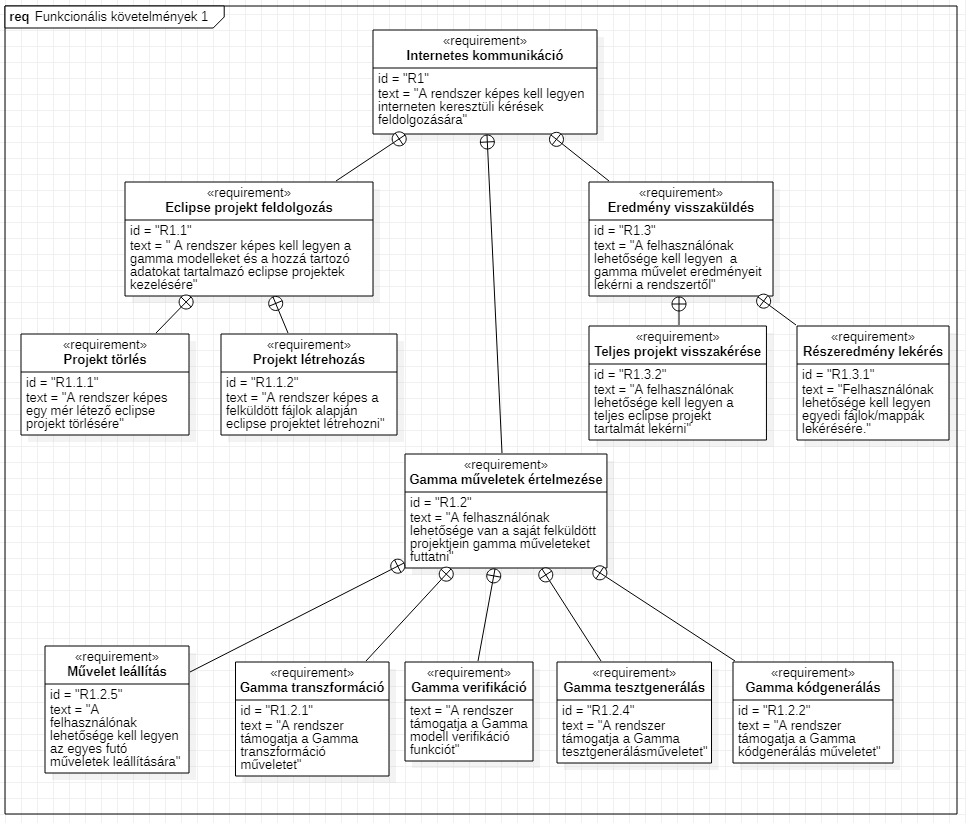
\includegraphics[width=\textwidth, keepaspectratio]{figures/requierments_placeholder.png}
	\caption{Követelmény hierarchia 1}
	\label{fig:requierments_placeholder}
\end{figure}

\begin{figure}[t]
	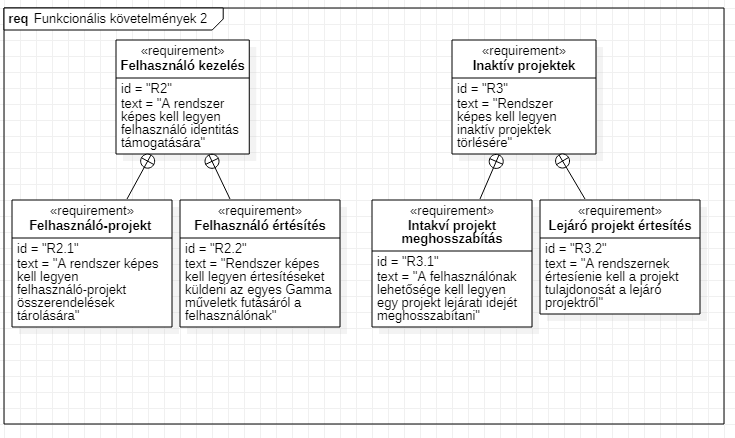
\includegraphics[width=150mm, keepaspectratio]{figures/requierments_2.png}
	\caption{Követelmény hierarchia 2}
	\label{fig:requierements_2}
\end{figure}

A további nem funkcionális követelményeket négy kategóriába soroljuk:
\begin{itemize}
	\item \textbf{Megbízhatóság:} Egy projekten nem futtathatunk két különböző Gamma művelet halmazt
	\item \textbf{Biztonság:} Minden felhasználó csak a saját projektjeit szerkesztheti / saját projektjein futtathat gamma művelet halmazokat / A rendszer képes kell legyen kiszűrni az egyes rosszindulatú felhasználók által megadott fájl elérési utakat / 
	\item \textbf{Teljesítmény:} A rendszer képes kell legyen különböző projekteken ugyanabban az időben Gamma műveletek futtatására. / A rendszer skálázható kell legyen. / A rendszernek nem szabad fölösleges adatot tárolnia. / A rendszer muszáj töröljön minden olyan adatot, amely neki vagy a felhasználó számára nem releváns. / A rendszer képes kell legyen asszinkron módban működni.
	\item \textbf{Felhasználhatóság:} A rendszer megfelelő, HTTP szabvány által előírt válaszokat adni az egyes kérésekre. / A rendszer beszédes értesítéseket kell küldjön a projekt tulajdonosának az egyes Gamma műveletek futási állapotáról.
\end{itemize}

A fentebb leírt követelmények alapján bizonyos technológiai döntéseket kellet hozni a projekt iniciális fázisaiban. Ahhoz, hogy az alkalmazásunk interneten keresztül is elérhető legyen egy webszervert kellet kialakítanunk, ez lesz a rendszer belépési pontja. A webszerver a REST API modern architektúra stílus szabályait betartva lett kialakítva. Mindez a \textit{R1.*} követelmény teljesítése teszi szükségessé. 

Ahhoz, hogy az \textit{R1.2.*} követelmény teljesüljön, a Gamma keretrendszert egy \textit{headless Eclipse}-be kellet becsomagolni. Ezzel megtudjuk oldani azt a problémát, hogy a Gamma az Eclipse IDE-hez van kötve, az így becsomagolt keretrendszert parancssoron keresztül lehet elérni.

Az \textit{R2.*} követelményt eclipse munkaterek (workspace) használatával teljesítjük. A rendszerünk biztosít munkatér létrehozás funkciót a felhasználói oldalon álló kliens szoftvernek, ehhez rendel egy egyedi azonosítót amit visszaküld a kliensnek és mostantól, ezzel az azonosító megadásával tud a kliens további funkciókat elérni. Mindezzel azt érjük el, hogy majdnem semmilyen információt nem kell tárolni a felhasználóról, ezt a feladatot rábízzuk a kliens szoftverre.

Összefoglalva a követelményeket és a technológiai döntéseket, olyan rendszert tervezünk, amely a Gamma keretrendszert elérhetővé teszi a világ számára, oly módon, hogy közben több felhasználói rendszerlogikát támogat az adatok tárolásán és funkciók elérésén. Továbbá, olyan mellék funkciókat is biztosítania kell, mint inaktív projektek automatizált törlése vagy felhasználók értesítése.

A rendszerben érdekelt személyek listája (\textbf{stakeholders}), azaz olyan aktorok, akik valamilyen módon kapcsolatba léphetnek a rendszerrel:
\begin{itemize}
	\item Komplex modellekkel foglalkozó \textbf{mérnökök} (NASA)
	\item \textbf{Egyetemi kutatók}
	\item Olyan \textbf{fejlesztő} aki integrálni akarja a rendszerünket egy harmadik párti alkalmazásba (MagicDraw)
	\item \textbf{Gamma fejlesztő} ,aki erőforrás igényes funkciót akar tesztelni
	\item \textbf{Üzemeltető}, aki a rendszer komponenseit frissíteni tudja
	\item \textbf{Üzleti oldalú kolléga}, aki a rendszert mint szolgáltatás hirdeti/eladja
\end{itemize}

A rendszer jelen formájában nem tartalmazza a fentebb többször említett kliens komponenst, így precíz használati eseteket nehéz definiálni. Ennek ellenére a rendszert teljes funkcionalitását lehet használni, tesztelni valamilyen API tesztelő szoftverrel, mint például PostMan. Olyan kéréseket tudunk küldeni az alkalmazás felé, amelyek teljes körűen szimulálják egy kliens szoftver viselkedését.

Az alapvető elérhető funkciók közé tartozik: a munkatér létrehozás, amely egy felhasználónak dedikált eclipse munkateret hoz létre, amin belül majd további műveleteket lehet végezni; eclipse projekt importálása archivált forrásból egy létező munkatérbe; az importált projektben szereplő, műveleteket leíró fájlok alapján gamma műveletek futtatása; a gamma műveletek által generált elemek visszakérése archivált fájlként; importált eclipse projekt törlése.


%----------------------------------------------------------------------------
\section{Architektúra}
%----------------------------------------------------------------------------

Ez a fejezet részletezi a specifikált rendszer struktúráját, továbbá áttekintünk fontosabb folyamatokat.
%----------------------------------------------------------------------------
\subsection{Struktúra}
%----------------------------------------------------------------------------

A rendszer felépítését \aref{fig:structure} ábra mutatja be. A továbbiakban részletezem az ábrán látható egyes komponenseket, milyen szerepük van és hogyan kommunikálnak más komponensekkel.
\begin{figure}[t]
	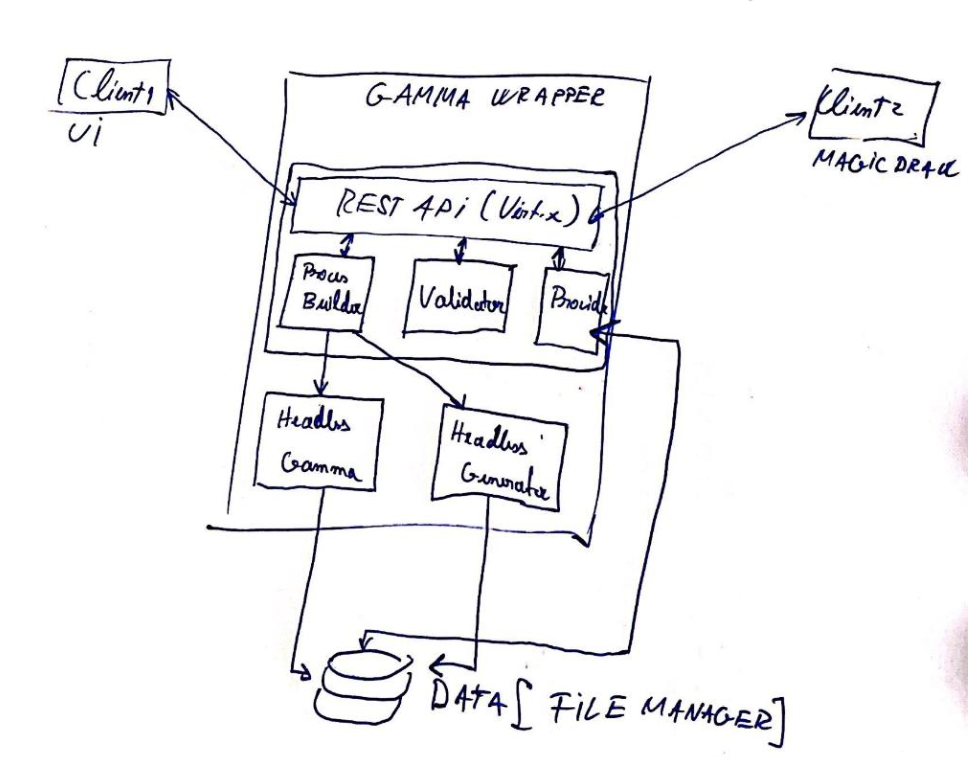
\includegraphics[width=150mm, keepaspectratio]{figures/architecture.jpg}
	\caption{Architektúra terv}
	\label{fig:structure}
\end{figure}
Az ábrán látható egy nagyobb, mindent magába foglaló \textit{Gamma Wrapper} nevezetű modul, ez a rendszer amely megvalósításra került a félév során és amiről a dolgozat szól. A nevét a funkcionalitásáról kapta, magyarul \textit{Gamma csomag}-nak is nevezhetnénk.

\paragraph{REST API} Ez az alkalmazás belépési pontja, ez látható a világ számára. Önmagában egy Vert.x webszerver amely egy OpenAPI specifikációban\footnote{OpenAPI specifikáció \url{https://app.swaggerhub.com/apis/szlnnn/GAMMA_WRAPPER3.0/1.0.0}} meghatározott \textit{endpoint}-ok alapján épül fel. Endpointnak hívjuk azokat az egyedi belépési pontokat, amelyek meghívhatók az alkalmazáson kívül. A rendszer az alábbi endpointokat tartalmazza, a fontosabbak működését a következő fejezet részletesen bemutatja:
\begin{itemize}
	\item POST /gamma/addworkspace eclipse workspace létrehozásának lehetőségét kínálja fel, minden további művelethez szükséges, a kérés nem tartalmaz további információt
	\item POST /gamma/addproject/{\textit{workspace}}\footnote{Minden döntött betűs rész egy URL-ben utazó paraméter} eclipse projekt létrehozást teszi lehetővé a {workspace} paraméterből kiolvasott munkatérben, a kérés törzsében szerepelnie kell az archivált fájl, ami tartalmazza az importálni kívánt projektet
	\item PUT /gamma/api/{\textit{workspace}}/{\textit{projectName}}/{\textit{filePath}} a munkatér és projekt páros alapján meghatározott Gamma műveleteket tartalmazó fájl futtatását teszi lehetővé. A {\textit{filePath}} paraméter írja le, hogy a műveleteket leíró fájl hol van, ez relatív kell legyen és a {\textit{projectName}} paraméterben tárolt projekt mappájában
	\item PUT /gamma/stopprocess/{\textit{workspace}}/{\textit{projectName}} a fentebb leírt folyamat leállítását teszi lehetővé, mivel egy projekt-munkatér pároson egy időben csak egy gamma művelethalmaz futhat ezért elég csak ezt a párost megadni
	\item PUT /gamma/getresult/{\textit{workspace}}/{\textit{projectName}} a gamma által generált fájlok visszakérését teszi lehetővé, ehhez szükséges, hogy a kérés törzsében utazzon, hogy milyen fájlokat/könyvtárakat szeretnénk visszakérni, az itt megadott elérések a projekthez képest relatívak kell legyenek, ha szerepel a "." elérés akkor a projekt teljes tartalmát visszaküldjük
	\item DELETE /gamma/deleteproject/{\textit{workspace}}/{\textit{projectName}} eclipse projekt törlését teszi lehetővé
	\item PUT /gamma/extendexpiration/{\textit{workspace}}/{\textit{projectName}} alapértelmezetten minden projekt automatikusan törlésre kerül 30 nappal a létrehozás után, ezzel az endpointal további 30 nappal lehet ezt az időtartamot meghosszabítani, az URL-ben utazó munkatér és projekt név párossal tudjuk eldönteni, hogy melyik projektet kívánja a felhasználó meghosszabbítani.
\end{itemize}
A komponens további feladatok is ellát, ilyenek a megfelelő HTTP válasz összeállítása, a szerverre küldött fájlok automatikus mentése vagy a más komponensek vezérlése. Egy időzítő is ide tartozik, ezzel ellenőrizzük a projektek lejárati dátumát és, ha ennek eljön az ideje akkor egy törlést fog indítani.

\paragraph{UI és MagicDraw} Mivel a rendszerünk egy szerver oldali komponens, ezért önmagában nem tudja bárki használni. Az ábrán feltüntetett kliens rendszereknek kell a felhasználói felület szerepét betölteni, ilyen lenne egy speciális UI ami az alapvető funkcióknak egy grafikus felületet biztosít és kontextust ad az alkalmazásunknak. Továbbá, tervben van a Gamma integrációja a MagicDraw\footnote{MagicDraw modellező eszköz \url{https://www.nomagic.com/products/magicdraw}} modellező eszközbe, a rendszerünk ezt az integrációt megkönnyítené. 

\paragraph{Headless Generator} A Gamma önmagában nem képes eclipse munkatér és projekt létrehozásra ezért kellet egy olyan komponens, ami előkészít egy környezetet, amiben futtathatunk Gamma műveleteket, ennek a neve \textit{Headless Generator}. Két fő funkciója van: eclipse munkatér (workspace) létrehozás és eclipse projekt importálás egy megadott munkatérbe. Mindkét funkcionalitást ugyanaz a folyamat valósítja meg annyi eltérésben, hogy ha a komponens kap egy archivált fájl elérést akkor tudni fogja, hogy ezt importálnia kell, mint eclipse projekt.  Egy \textit{headless runtime eclipse}-ként van megvalósítva és parancssorból lehet meghívni, két paramétert lehet megadni az első a \textit{-data} amiben a workspace nevét kell megadni, ha egy nem létező workspace-t adunk meg akkor a komponens ezt létrehozza, ez egy kötelező paraméter. A második argumentum pedig a projekt archivált fájl elérése, ezt fogja kicsomagolni és regisztrálni a munkatérbe, ez az argumentum opcionális. Fontos kiemelni, hogy a forrás fájl már a munkatér mappájában kell legyen.

\paragraph{Headless Gamma} Annak ellenére, hogy csupán egy endpoint meghívása során kerül működésbe a rendszer legfontosabb eleme. A Headless Generator-hoz hasonlóan egy headless runtime eclipse-ként lett kialakítva és ugyanúgy parancssorból lehet elindítani. Három kötelező paraméterre van szüksége. (1) Létező munkatér, amely tartalmazza az átadott (2) projekt állományait. Az utolsó (3) paraméter egy a projekthez relatív elérés, ami a gamma műveleteket leíró fájlra mutat. A fájl .ggen kiterjesztésű kell legyen, és megfelelő sorrendbe kell tartalmazza a futtatni kívánt műveleteket és a futtatáshoz szükséges modell állományok hivatkozását, amelyek a projekten belül kell legyenek. A Gamma miután elvégezte a műveleteket tipikusan 3 mappába generálja le az eredményeket: src-gen,test-gen, trace. Ezek mind a projekt mappán belül találhatóak. 

Az UPAAL telepítése egy alapvető követelmény a gamma megfelelő működéséhez, ennek az elérést a rendszer a környezeti változókból tudja kinyerni.
Az OSGi előnyeit itt tudjuk kihasználni, mivel a headless gamma több száz \textit{plug-in}-t igényel. A plug-in-ek egyesével frissíthetőek, elméletileg nem kéne nagy akadályt okozzon egy új release telepítése.

\paragraph{Process Builder} A REST webszerver és a headless komponensek közé biztosítani kell egy olyan réteget, ami a webes hívások paramétereit átalakítja parancssori argumentumokká és eltud indítani egy ilyen runtime eclipse-t, ezt a szerepet a \textit{Process Builder} tölti be. Négy funkció esetén jelenik meg a végrehajtási sorban, (1) munkatér létrehozás, (2) projekt importálás archív fájlból, (3) gamma művelet futtatás és (4) gamma műveletet futtató folyamat leállítás. Minden funkció esetén lehetőség van asszinkron működésre, viszont jelenleg csak a (3) és (4) esetén van implementálva,  a szinkron működést azzal az érvel lehet védeni, hogy csak abban az esetben küldjünk választ a kliensnek ha valóban a kért funkcionalitást eltudtuk végezni. Ez a gamma művelet futtatáskor azért nem egy élhető koncepció, mert vannak olyan modellek amelyek több ezer vagy akár több tíz ezer állapotból állnak, ezeknek a feldolgozása órákba is kerülhet így az asszinkron működés egy szükséglet. A gamma művelet leállítása pedig nem igényel semmilyen megvárást, nincs olyan eset amikor ez eltud akadni. A másik két esetben (1)(2) viszont megvárjuk amíg a munkatér vagy projekt létrejön, mert nem költséges műveletek, ezt a jövőben érdemes lehet átgondolni és esetleg átalakítani.
\paragraph{Validator} A valamennyi bejövő kérések validációs lépéseken is át kell essenek, ezt a \textit{Validator} modul biztosítja. A REST webszerver vezérli, hogy a bejövő paraméterek közül melyek azok amelyek valamilyen validáción át kell essenek. A legfontosabb ellenőrzési lépések közé tartoznak a munkatér létezés ellenőrzése, a projekt-munkatér páros vizsgálata és az átadott projekten futó gamma folyamat ellenőrzése. Az utóbbi kiemelkedően fontos, hiszen egy futás alatt levő projekttel nem végezhetünk semmit, csak leállíthatjuk. Ahhoz, hogy a futás állapotát nyilván tudjuk tartani, be lett vezetve egy leíró json fájl amit minden projekt importálásánál létrehozunk, ez a fájl többek közt tartalmazza azt is, hogy jelenleg van-e futó folyamat a projekten. Ennek az állapotát a ProcessBuilder beállítja \textit{inProgress}-be majd a HeadlessGamma futása végén frissíti \textit{notInProgress}-re.
\paragraph{Provider} A \textit{Provider}-nek két feladat van, az első, hogy a REST webszerver által feldolgozott eredmény visszakérő endpoint-ban megadott relatív elérések alapján összecsomagoljon egy zip állományt, a másik pedig a projekt törlés. Az eredmény fájl összecsomagolásánál lehetőségünk van megadni egyedi fájlok elérését vagy akár teljes mappákat. Ide tartozik a teljes projekt mappa is, ezt a "." eléréssel tudjuk megadni, ha ez szerepel a kérésbe akkor a többi eredmény eléréssel nem is foglalkozik a rendszer, hiszen ez mindent tartalmazni fog.
\paragraph{Data} Az ábrán megjelenik a \textit{Data} fogalom is, ez valójában a hoszt szerveren levő fájl kezelőt jelenti. Itt tároljuk a létrehozott munkatér és projekt párosokat és ezek teljes tartalmát, továbbá a metaadatokat tároló json fájlokat is. Egy adatbázis réteg bevezetésével a fájlban tárolt metaadatokat könnyebben tudnánk kezelni, sajnos a projektbe ez nem fért bele.



%----------------------------------------------------------------------------
\subsection{Folyamatok}
%----------------------------------------------------------------------------

Négy alapvető funkció részletes működését fogom bemutatni ebben a fejezetben, ezek sorra: munkatér létrehozás, projekt importálás, gamma műveletek futtatása és a futtatás eredmény lekérés. A folyamat bemutatja milyen modulokon megy végig az adat, továbbá milyen feldolgozások történnek egyes végrehajtási lépéseken. Mindezt szekvencia diagramokkal ábrázoltam. Az így bemutatott funkciók lefedik a rendszer legfontosabb felhasználói eseteit.


\paragraph{Munkatér létrehozás}

\begin{figure}[!ht]
	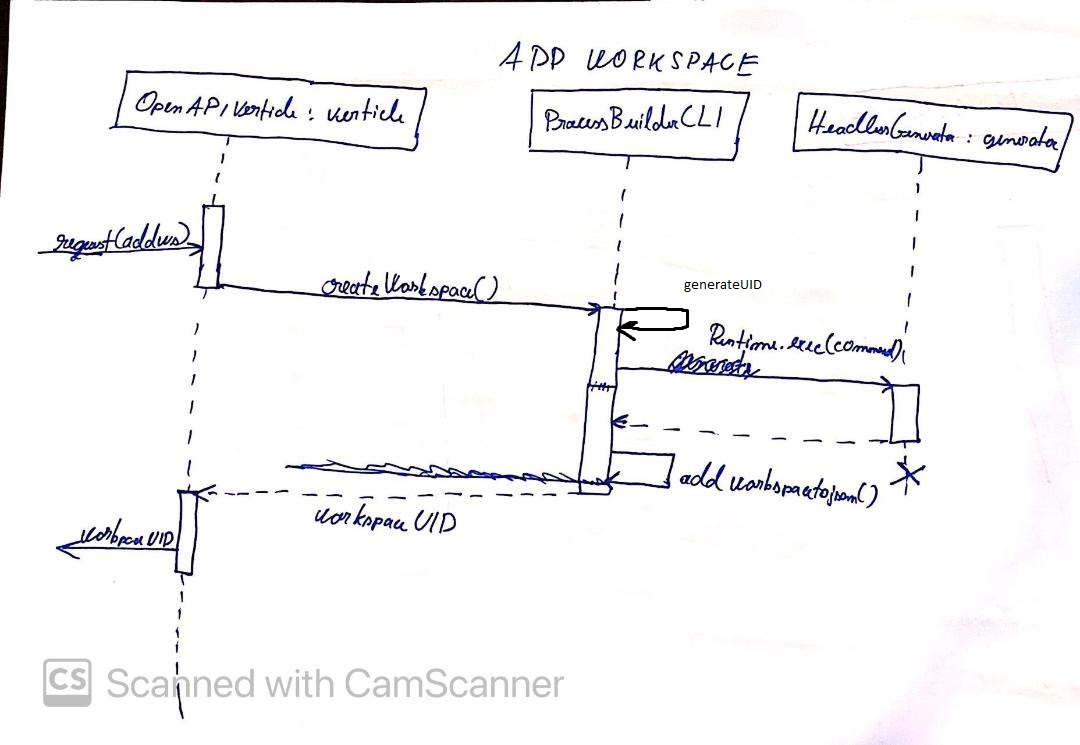
\includegraphics[width=150mm, keepaspectratio]{figures/add_workspace_seq.jpg}
	\caption{Munkatér létrehozás szekvencia diagram}
	\label{fig:addworkspace}
\end{figure}

A workspace létrehozás szekvencia diagramja \aref{fig:addworkspace} ábrán látható. Első fázisban bejön egy POST HTTP metódus az addworkspace endpointra, ennek a törzse üres és az URL-ben sem hordoz paramétereket. Látható, hogy az OpenAPIVerticle fogadja a kérést, ez lényegében a REST webszerverünk, mivel ez a legelső művelet, amit a kliens meg kell hívjon így nem kell semmilyen ellenőrzést végezni. A végrehajtási sor következő lépése a \textit{ProcessBuilder}-ben van, itt a rendszer generál egy egyedi UID azonosítót, amit felhasznál a parancs kialakításhoz, amivel elindítja a a HeadlessGenerator-t.A parancs (command) elkészítéséhez a ProcessBuildernek szüksége van a headless eclipse elérésére, ezt a \textit{config.properties} fájlban lehet beállítani. A generator amíg elkészíti a workspace-t a ProcessBuilder vár, ha végzett akkor visszaadja az OpenAPIVerticle-nek a generált UID-ot ami továbbítja a kliens felé. Mikor a headless eclipse elvégezte a feladatot akkor teljesen leáll, ezt jelzi az X a folyamatábrán.


\paragraph{Eclipse projekt importálás}
\begin{figure}[!ht]
	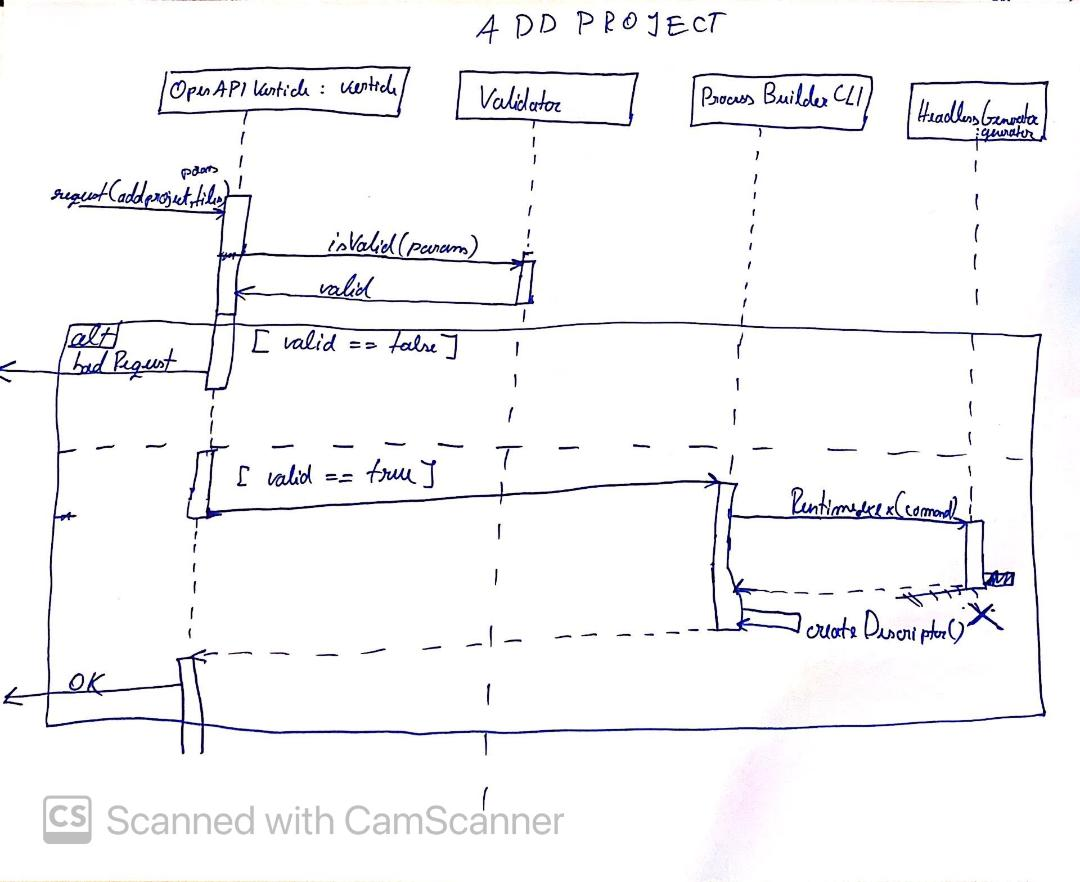
\includegraphics[width=150mm, keepaspectratio]{figures/add_eclipseproject_seq.jpg}
	\caption{Eclipse projekt importálás szekvencia diagram}
	\label{fig:addproject}
\end{figure}

A projekt importálás funkció szekvencia diagramját \aref{fig:addproject} ábrán lehet megtekinteni. A folyamat megint a kérés érkezésével indul, ezt minden esetben az OpenAPIVerticle dolgozza fel, ez a kérés egy POST HTTP metódus ami az addproject endpoint-ra jön be. Ebben az esetben viszont már az URL-ben utazik egy munkatér azonosító amit korábban adtunk vissza a workspace létrehozáskor. Továbbá, a törzsben két attribútum szerepel: (1) \textit{files} ez tartalmazza a projekt archivált állományait és (2) \textit{contact} ez egy email cím, ami a projekt tulajdonosáé, erre későbbiekben értesítések küldésénél lesz szükségünk. A munkatér létezését a Validator komponenssel elvégezzük, a kapott válasz alapján két esetet különböztetünk meg, az első, ha nem érvényes a megadott workspace azonosító, ekkor egyből szólunk a kliensnek, hogy rossz a kérés. Viszont, ha ez helyes akkor tovább adjuk a kérést a ProcessBuilder-nek ami az előző esethez hasonlóan elindítja a HeadlessGenerator-t, de kiegészíti az argumentum listát a forrás fájl nevével, mindezek előtt a nyers fájlt a munkatér mappájába másolja. A generator elvégzi az import műveletet, majd visszaadja a futási jogot a ProcessBuildernek, ami végezetül regisztrálja a munkatér-projekt párost és létrehoz egy leíró fájlt a frissen létrehozott projektben, ami tartalmazza, hogy mi a projekt neve, ki hozta létre (email cím), mikor hozta létre, mikor jár le és beállítja, hogy jelenleg nincs futás alatt, ezek után törli az iniciális forrás fájlt, hogy tárhelyet spóroljunk. Végezetül visszaadja a futási jogot a verticle-nek aki jelez a kliensnek, hogy minden rendben létrejött.



\paragraph{Gamma műveletek futtatása}
\begin{figure}[!ht]
	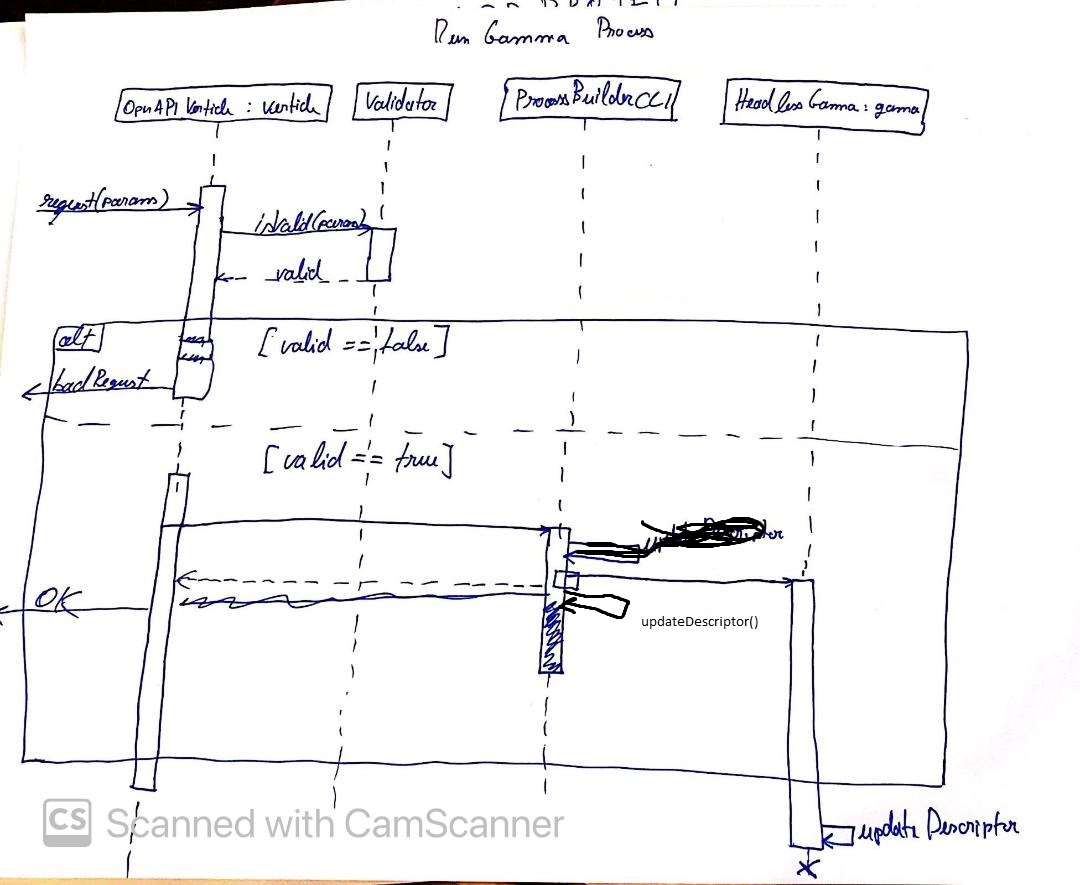
\includegraphics[width=150mm, keepaspectratio]{figures/run_gamma_seq.jpg}
	\caption{Gamma művelet futtatás szekvencia diagram}
	\label{fig:rungamma}
\end{figure}
A gamma műveletek futtatását bemutató szekvencia diagram \aref{fig:rungamma} ábrán tekinthető meg. Ebben az esetben egy PUT HTTP kérés érkezik az \textit{api} endpoint-ra, amit szintén az OpenAPI réteg dolgoz fel kezdetben. A törzsben nem szerepel semmi, viszont az URL-ben utazik a munkatér azonosító, projektnév és futtatni kívánt gamma műveleteket leíró .ggen fájl elérése. Ez a hármas egyedileg meghatározza az erőforrást. A validációs fázis komplexebb ebben az esetben, hiszen ellenőriznünk kell a munkatér-projekt páros létezését és egyediségét, mert egy projekt egyszer szerepelhet egy munkatérben, továbbá azt is meg kell vizsgálni, hogy a projekt, amit ez a páros leír jelenleg használva van-e valamilyen más gamma műveletet futtató headless eclipse által. A Validator döntése alapján, megint két esetet különböztetünk meg, ha valamiért nem felel meg akkor az OpenAPIVerticle a megfelelő hibakóddal és üzenettel visszaszól a kliensnek, hogy nem érvényes a kérés. Ha minden megfelel, akkor a futást átadjuk a ProcessBuilder-nek, ami asszinkron módon elindítja a gamma műveletet futtató headless eclipset. Ezek után egyből frissíti a projektet leíró fájlt, pontosabban, rögzíti az így elindított folyamat operációs rendszer szintű azonosítóját (PID) és beállítja, hogy a projekt futás alatt van. Végezetül átadja a futást a verticle-nek, ami jelzi a kliens felé, hogy a kérés feldolgozása elkezdődött.
A folyamat még nem ér véget, mivel a Gamma dolgozik a háttérben, mikor minden művelet lefutott amit a .ggen fájlban meghatározott a felhasználó, akkor a headless eclipse frissíti a projektet leíró állományt és beállítja, hogy a projekt már nincs futás alatt. További lezáró művelet lehet az értesítés küldés a tárolt email címre, hogy a kért kérés lefutott és az eredmény mostantól lekérhető.


\paragraph{Eredmények lekérése}
\begin{figure}[!ht]
	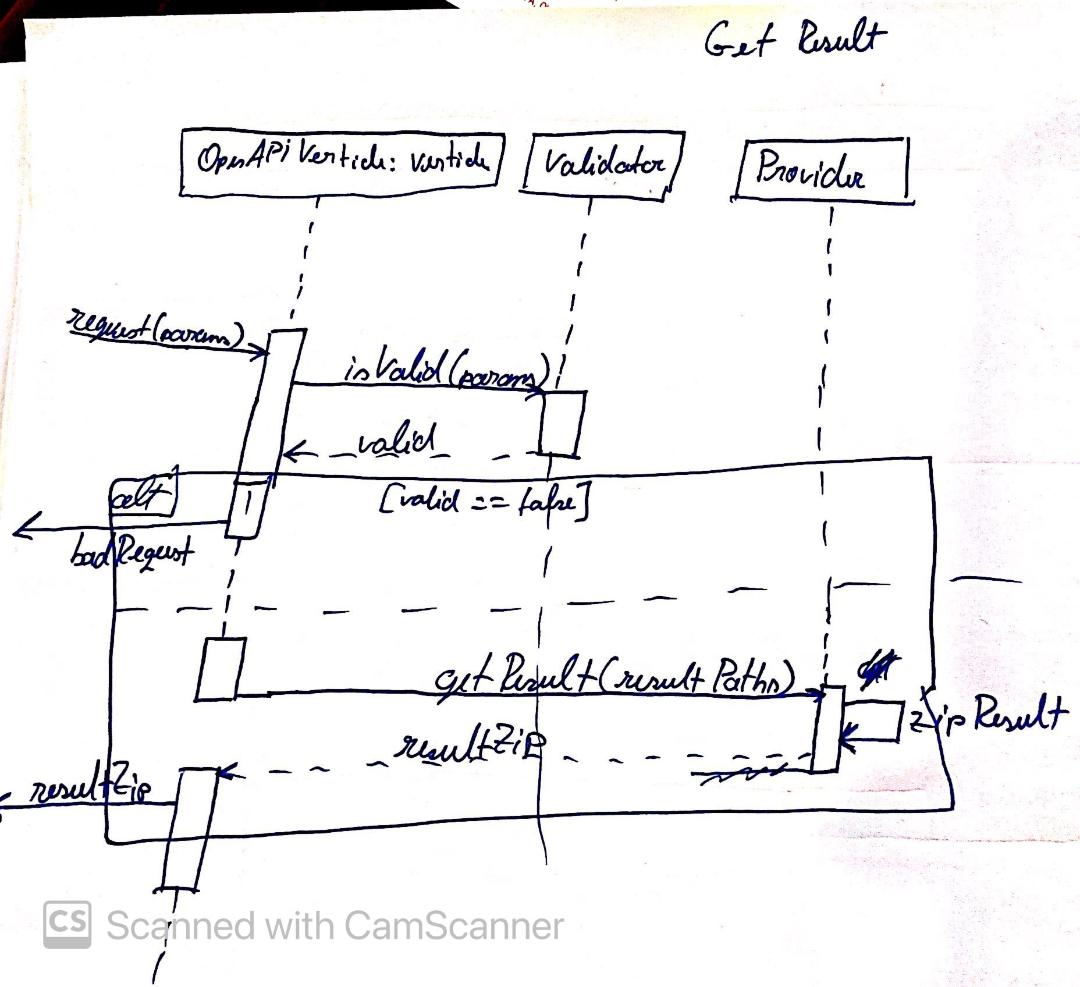
\includegraphics[width=150mm, keepaspectratio]{figures/get_result_seq.jpg}
	\caption{Eredmény lekérés szekvencia diagram}
	\label{fig:getresult}
\end{figure}
A gamma által generált állományok lekérésére szolgáló funkció szekvencia diagramját \aref{fig:getresult} ábra mutatja be. Egy PUT HTTP kérés érkezik a \textit{getresult} endpoint-ra, ennek az URL-jében szerepelnie kell a munkatér azonosítójának és a projektnévnek amiből adatot akarunk lekérni. A kérés törzsében a \textit{resultDirs} attribútum kell szerepeljen, ami egy relatív elérésekből álló lista. A kérés feldolgozása a szokásos módon a verticle-ben kezdődik, ahol a kérésben utazó paraméterek kicsomagolásra kerülnek. A Validator ebben az esetben ugyanazokat ellenőrzi, mint a művelet futtatás folyamat esetén. Ha van futó folyamat a projekten vagy a workspace projekt páros nem megfelelő, akkor beszédes hibaüzenettel válaszolunk a kliensnek. Abban az esetben, ha minden rendben van, akkor a Provider kapja meg  a futási jogot. Itt az elérési listán iterálva összegyűjtjük a kért fájlokat és mappákat majd archiváljuk, az így archivált fájl elérést küldjük vissza a verticle-nek, ami ennek alapján visszaküldi a fájlt.

Első látszatra zavaró lehet, hogy PUT metódust használunk a kérés feldolgozásához, mikor egy GET jobb lehetne és jobban megfelelne a REST szabványnak. Ennek két oka van, az első az, hogy annak ellenére, hogy \textit{getresult}-nak hívjuk az endpoint-ot az erőforrás állapota módosul hiszen a projekten belül generálunk egy archivált fájlt, a másik oka pedig az, hogy a GET kérésnél nem lehet a törzsben semmit sem küldeni, ezt a REST szigorúan megköveteli, nekünk viszont a becsomagolni kívánt állományokat listában kell megadnunk és ezt az URL-ben kényelmetlen lenne kezelni.


%----------------------------------------------------------------------------
\section{Implementáció}
%----------------------------------------------------------------------------

%----------------------------------------------------------------------------
\subsection{Fejlesztés folyamata}
%----------------------------------------------------------------------------


Ebben a fejezetben a fejlesztés során felmerült nehézségeket és érédességeket mutatom be. Az alábbi információk alapvetően mély technikai szintre lemennek így szárazak lehetnek, viszont a témában dolgozóknak hasznos lehet, mert egyedi hibák és jelenségek megoldását vázolom föl.

\paragraph{Eclipse környezettel kapcsolatos érdekességek} Az Eclipse környezetben tapasztalt fejlesztők tudják, hogy bizonyos dolgok nem triviálisak a fejlesztés során és olyan specifikus problémák merülhetnek fel, amelyekre nagyon elrejtett internetes fórumokon lehet választ kapni. Az alábbi jelenségek és problémák a \textit{Headless Gamma} komponens fejlesztése alatt merültek föl

Az eclipse plug-in fejlesztés és termék export konfiguráció során számos függősségi problémával szembesültem. A legelső érdekesség ami felmerült, az volt, hogy az Eclipse a \textit{product} konfigurációban meghatározott plug-in függőségek verzióját automatikusan felülírta a környezetbe telepített legfrissebb verzióval. Ezen plug-in-ek listáját az Eclipse IDE-n belül a \textit{Target Platform}-on lehet megtekinteni és szerkeszteni. Ilyen problémás függőségek voltak a \textit{batik.css} és \textit{batik.util} plug-in-ek. A Target Platform szerkesztésével ezt a problémát orvosolni lehet, csupán ki kell vegyük vagy hozzá kell adjuk azt a verziót amire szükségünk van és győződjünk meg, hogy az adott plug-in-ből csak egy verziót aktív.

A product konfigurációban a \textit{Content} fülön tudjuk meghatározni milyen plug-in-ekből álljon a termékünk, az IDE-ben lehetőség van arra, hogy megadjuk a fejlesztett alkalmazásunkat és rányomva az \textit{Add Requiered} gombra az IDE automatikusan beállítja a termékünk összes függőségét. Ennek ellenére az osgi.extender olyan plug-in-eket igényel, amelyek az OSGi helyes működéséhez szükségesek de nem importálja be automatikusan. A szükséges modulok:
\begin{lstlisting}[language=]
org.apache.felix.scr
org.eclipse.equinox.event
org.eclipse.compare.core
org.eclipse.fx.osgi
org.eclipse.team.core
\end{lstlisting}

Olyan jelenség is előjött, ahol a függőségi fában egy plug-in kétszer szerepelt viszont különböző verzióval, ezt az OSGi szabvány engedi de az Eclipse, az első jelenségben leírtak alapján, folyamatosan felülírta az elavultabb verziót. A probléma elképzelésében segít  \aref{fig:depend} ábra. Erre a megoldás az, hogy a fában felfele haladva megvizsgáljuk, hogy milyen verziókat tudunk frissíteni a Target Platformon úgy, hogy a működést megtartsuk de az elavult verziójú plug-in-t frissíteni tudjuk. Alapvetően egyszerű feladatnak tűnik, viszont a rendszer közel 250 függőséggel rendelkezik.

\begin{figure}[t]
	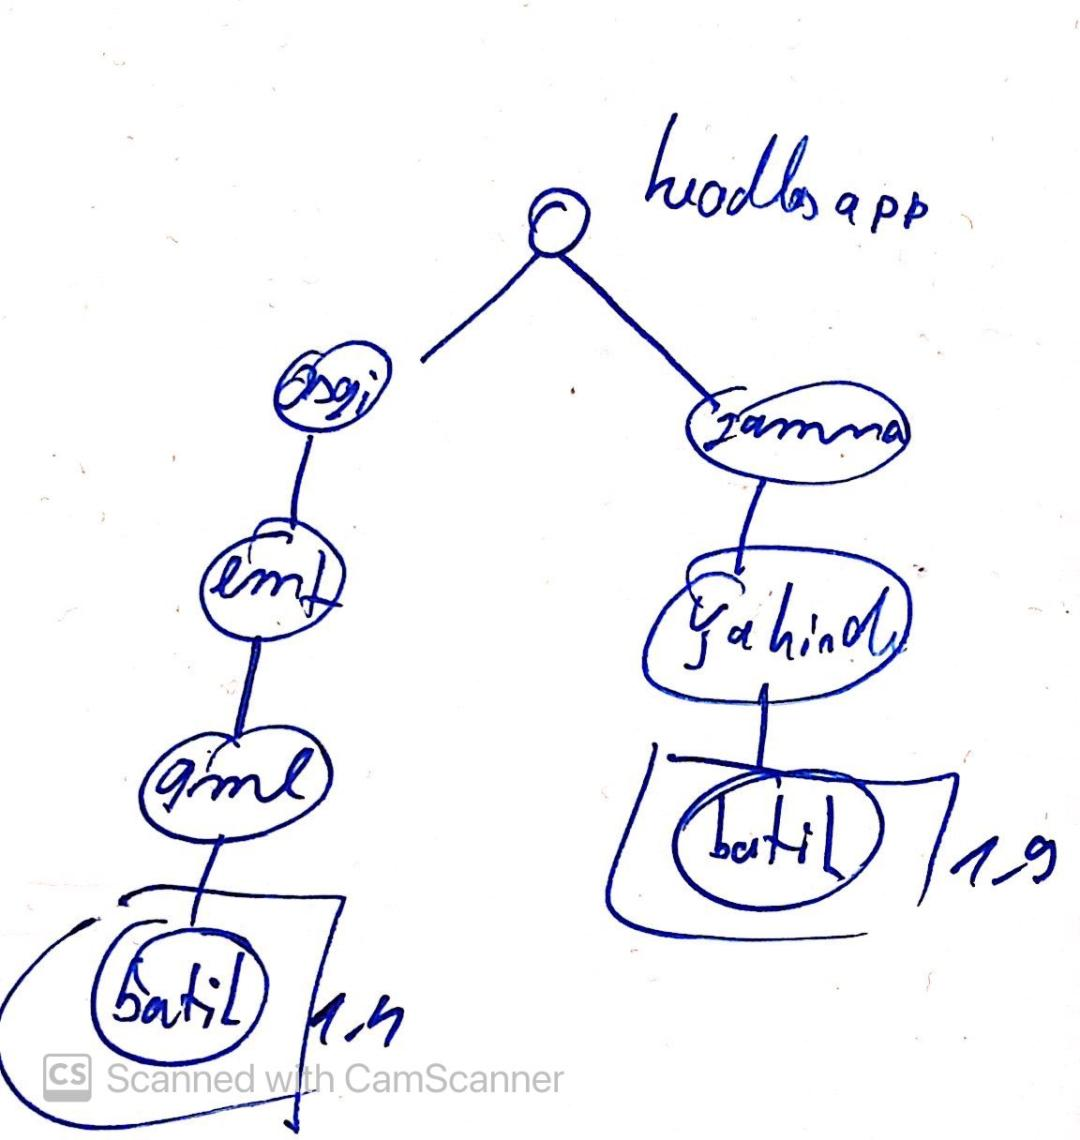
\includegraphics[width=150mm, keepaspectratio]{figures/depend.jpg}
	\caption{Egyszerűsített függőségi fa}
	\label{fig:depend}
\end{figure}

A termék export felületen meg kell határozni, hogy az egyes Eclipse modulok milyen sorrendbe induljanak el, a mi esetünkbe az alábbi indulási szintek meghatározása volt fontos:
\begin{lstlisting}[language=XML]
<configurations>
	<plugin id="org.apache.felix.scr" autoStart="true" startLevel="2" />
	<plugin id="org.eclipse.core.runtime" autoStart="true" startLevel="0" />
	<plugin id="org.eclipse.equinox.common" autoStart="true" startLevel="2" />
	<plugin id="org.eclipse.equinox.event" autoStart="true" startLevel="2" />
	<plugin id="org.eclipse.equinox.simpleconfigurator" autoStart="true" startLevel="1" />
</configurations>
\end{lstlisting}
Ez a konfiguráció részlet a termék leírás XML fájlból van másolva, az IDE-ben a \textit{Configuration} fülön lehet mindezt beállítani.

Egy termék konfiguráció futtatására két lehetőségünk van, az első, hogy exportáljuk (headless eclipse) majd parancssorból meghívjuk és átadjuk az argumentumokat vagy az IDE-ből elindítjuk. Az utóbbi tesztelés folyamán nagyon hasznos tud lenni. Ha IDE-ből futtatjuk akkor is van lehetőségünk argumentumokat átadni, erre szintén a termék konfigurációban van lehetőség, pontosabban a \textit{Launching} fülön. Arra viszont érdemes odafigyelni, hogy ezt a tesztelés után ne hagyjuk ott, mivel az export konstans argumentumoknak értelmezi és minden headless módban indulásnál átadja önmagának. A mi esetünkbe ez hatványozottan fontos, mivel az átadott argumentumok minden esetben mások a munkatér és projektek számossága miatt.

Minden függőség lehet opcionális vagy kötelező az opcionálisakat csak abban az esetben tölti be a headless eclipse mikor éppen szüksége van rá. A rendszerünknek a \textit{jdt} plug-in család több komponensére is szüksége van viszont ezek a függőségi fában levő szülőjükön a \textit{xtext.ui} plug-in-en csupán opcionálisként vannak megjelölve és egy mai napig nem tisztázott ok miatt nem töltődtek be. A problémát azzal lehet orvosolni, hogy készítünk az xtext.ui plug-in-ből egy saját példányt, amin a függőségi beállításokat átírjuk opcionálisról kötelezőre. Ez sajnos nehezíti a rendszer tovább fejlesztését és a telepítési folyamat is komplexebbé válik.

Egy kulcsfontosságú probléma az volt, hogy az Xtext\footnote{Xtext-ről többet: \url{https://www.eclipse.org/Xtext/}} modult eddig nem tudtuk injektálni a headless eclipse-be. Erre az alábbi kódrészlet ad megoldást:
\begin{lstlisting}[language=Java]
 	Injector injector = new StatechartLanguageStandaloneSetupGenerated()
 							.createInjectorAndDoEMFRegistration();
 	XtextResourceSet resourceSet = injector.getInstance(XtextResourceSet.class);
\end{lstlisting}
A fent definiált \textit{resourceSet}-ről tudjuk majd a headless eclipse-nek argumentumban átadott fájlt elérni.

Minden Gamma nyelv interpretálóját egyedileg meg kellet hívni az alkalmazás indulási pillanataiban:

\begin{lstlisting}[language=Java]
//Alkalmazás belépési pontja
 @Override
public Object start(final IApplicationContext context) throws Exception {
	ExpressionLanguageStandaloneSetup.doSetup();
	ActionLanguageStandaloneSetup.doSetup();
	StatechartLanguageStandaloneSetup.doSetup();
	TraceLanguageStandaloneSetup.doSetup();
	PropertyLanguageStandaloneSetup.doSetup();        
	GenModelStandaloneSetup.doSetup();
	.
	.
	.
}
\end{lstlisting}

\paragraph{OpenAPI REST webszerver} Olyan fejlesztői megoldásokat mutatok be, amelyek az OpenAPI és Vert.x használata által nagyon egyszerűen megvalósíthatóak voltak. Ehhez tekintsük át \aref{fig:endpoint_example} ábrát amely az \textit{addproject} endpoint specifikációját tartalmazza.

A Vert.x, mint említettem támogatja az OpenAPI REST specifikáció integrációját, így kódból az alábbi módon tudjuk elérni a fájlban definiált \textit{endpointot} (gamma-wrapper.yaml), amit majd regisztrálunk a webszerverünkbe:
\begin{lstlisting}[language=Java]
@Override
public void start(Future<Void> future) {
        OpenAPI3RouterFactory.create(this.vertx, "gamma-wrapper.yaml", ar ->
		{
               	OpenAPI3RouterFactory routerFactory = ar.result();
                routerFactory.addHandlerByOperationId("addProject", routingContext -> {	... });
				...	
		});
}
\end{lstlisting}
A fenti kódrészletben már nagyon egyszerűen tudjuk a kérésben utazó paramétereket Java objektummá átalakítani.A példában fájlok feldolgozását is el kell végezzük, ezt a Vert.x a fenti \textit{routingContext} objektumon már eltárolja és egy egyszerű \textit{routingContext.fileUploads()} hívással már \textit{File} objektumok listáját kapjuk vissza.


Bizonyos validációs feladatokat is elvégez helyettünk az OpenAPI definíció alapján a Vert.x, \aref{fig:endpoint_example} ábrán látható, hogy meghatározzuk a munkatér(workspace) szintaktikáját, ha ettől eltérő, más formátumú karakterlánc szerepel a kérésben akkor automatikusan küldődik egy válasz a klienshez, hogy nem megfelelő a kérése.



\begin{figure}[!ht]
	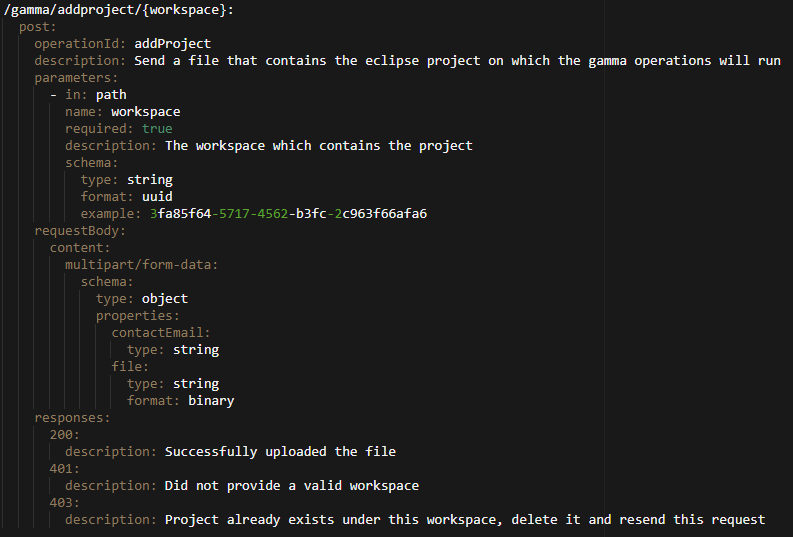
\includegraphics[width=150mm, keepaspectratio]{figures/endpoint_example.png}
	\caption{Endpoint példa}
	\label{fig:endpoint_example}
\end{figure}

\paragraph{ProcessBuilder fejlesztés} Alapvetően a webszerver java 8 alapokon lett megvalósítva, majd kiderült, hogy a java 9 hasznos, új frissítéseket tartalmaz a \textit{java.lang.ProcessBuilder} komponensén. Számunkra ez azért fontos, mert bevezetésre került a \textit{pid} (process id) lekérése az éppen indított folyamatról. Ezt az azonosítót feltudjuk használni, hogy egy Gamma műveleteket feldolgozó folyamatot leállítsunk, ha úgy gondoljuk, hogy túl sok ideig fut.
Nagyon fontos megjegyezni azt, hogy ha folyamatot indítunk a \textit{java.lang.ProcessBuilder} segítségével és ez több ideig fut, akkor a logolási eredményét kötelezően át kell irányítsuk fájlba vagy konzolba. Ennek hiányában a folyamatunk beakad. A rendszerünk a folyamatot indító konténerre leörökölteti a logolás feladatát. A HeadlessGamma elindítására szolgáló kódrészlet:

\begin{lstlisting}[language=Java]
	ProcessBuilder pb = new ProcessBuilder(commandToBeExecuted); // ProcessBuilder inicializálás, commandToBeExecuted a futtatni kivánt parancs karakterláncát tartalmazza
	pb.redirectErrorStream(true);
	pb.inheritIO(); // Logolás öröklés
	long pib =  pb.start().pid(); // Folyamat azonosító lekérése
}
\end{lstlisting}


%----------------------------------------------------------------------------
\subsection{Rendszer szoftverkomponensei}
%----------------------------------------------------------------------------

A rendszer struktúrájából kiindulva, ezt \aref{fig:structure} ábrán lehet megtekinteni, a rendszer szoftver szintű felépítése három komponensből tevődik össze, ezek vizuális reprezentációját \aref{fig:software_components} ábra mutatja be.

\begin{figure}[t]
	\centering
	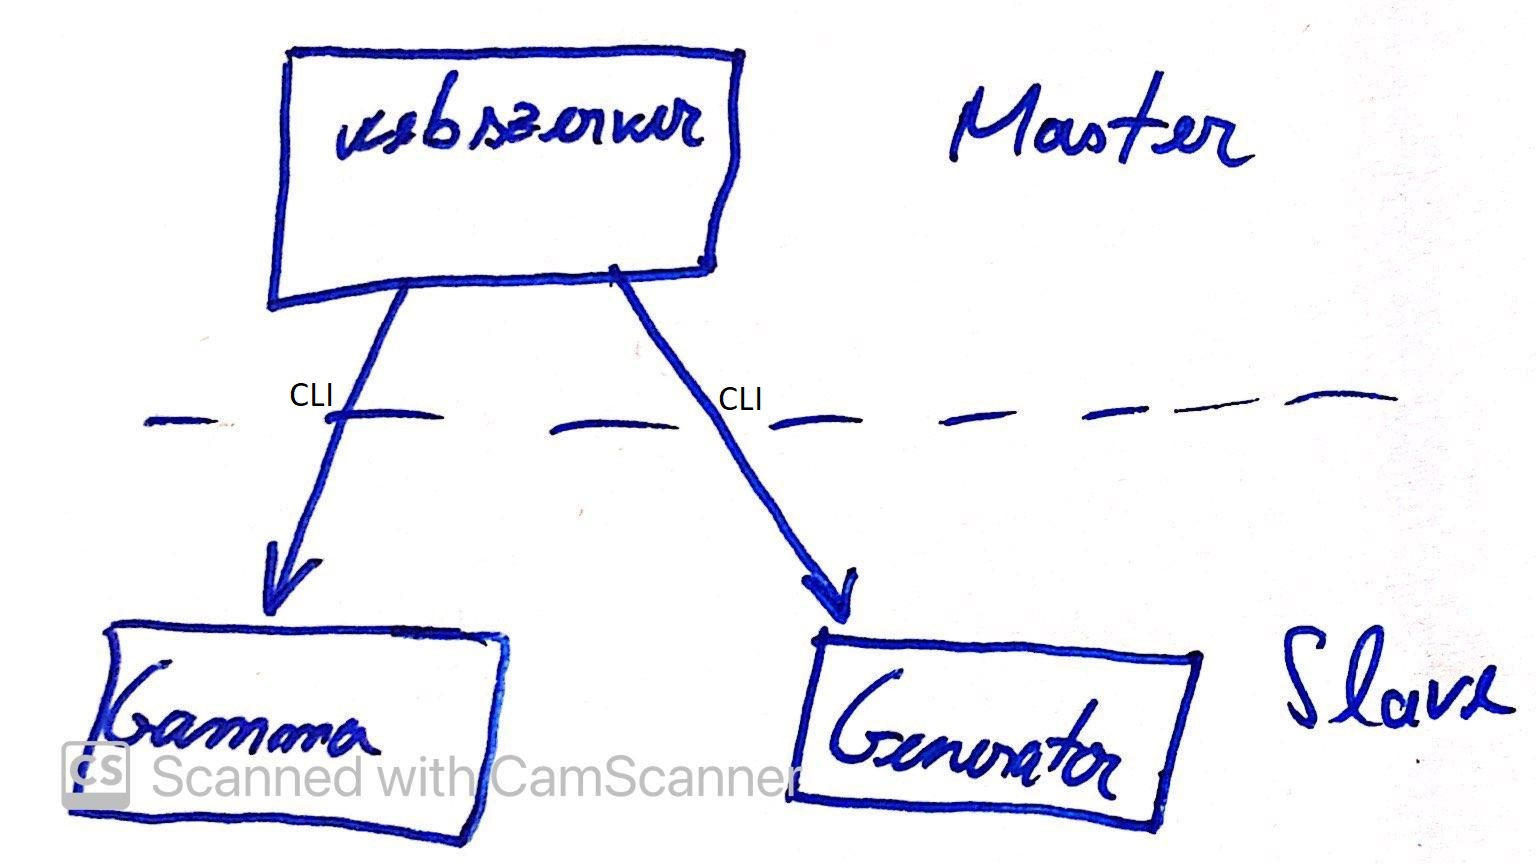
\includegraphics[width=75mm, keepaspectratio]{figures/software_components.jpg}
	\caption{Szoftver komponensek}
	\label{fig:software_components}
\end{figure}

A Webszerver tartalmazza az összes olyan komponenst, amely a webes kérések értelmezését és átalakítását végzik, itt található az OpenAPI definíció. Önmagában egy Maven\footnote{Maven-ről többet: \url{https://maven.apache.org/}} alapú InteliJ IDEA-ban fejlesztett alkalmazás. A Gamma és a Generator pedig az eddigiekben már többször említett két headless eclipse alkalmazás. A webszerver egy master szerepet tölt be a rendszerünkbe, mivel ö koordinálja a másik kettő működését.
